%%% Intro chapitre 2
\chapter{Système de recommandation}
\section*{Introduction}
\phantomsection
\addcontentsline{toc}{section}{Introduction}
\paragraph{}
Les systèmes de recommandation sont une forme spécifique de filtrage d’information visant à
présenter les éléments d'information qui sont susceptibles d'intéresser l'utilisateur. Ils peuvent être
définis comme des programmes qui tentent de recommander les articles (produits ou services) les
mieux adaptés à des utilisateurs particuliers (particuliers ou entreprises) en prévoyant l'intérêt d'un
utilisateur pour un article en fonction d'informations connexes sur les articles, les utilisateurs et les
interactions entre eux (Bobadilla et al., 2013).

L’élaboration de systèmes de recommandation a pour objectif de réduire la surcharge
d’informations en récupérant les informations et les services les plus pertinents à partir d’une
quantité énorme de données, fournissant ainsi des services personnalisés. La caractéristique la plus
importante d'un système de recommandation est sa capacité à « deviner » les préférences et les
intérêts d'un utilisateur en analysant le comportement de cet utilisateur et / ou celui d'autres
utilisateurs pour générer des recommandations personnalisées (Resnick \& Varian, 1997).

Les systèmes de recommandation ont été définis de plusieurs façons. La définition la plus populaire
et la plus générale que nous citons ici est celle de Robin Burke (Burke, 2002) :
Un système de recommandation est : « un système capable de fournir des recommandations
personnalisées ou permettant de guider l’utilisateur vers des ressources intéressantes ou utiles au
sein d’un espace de données important ».

Dans tout système de recommandation, il existe deux entités qui représentent le cœur du système.
Toute technique de recommandation tourne autour de ces entités qui sont : les utilisateurs et les
items.

L’utilisateur est la personne qui interagit avec le système, à qui le système recommande des items
et à son tour donne son avis sur les items.

L’item est le terme général utilisé pour désigner la ressource que le système suggère aux
utilisateurs.

Avec l’utilisateur et l’item, le domaine d’information d’un système de recommandation contient
aussi une préférence exprimée par un utilisateur pour un item qui est appelée note, et est souvent
représentée par un triplet (utilisateur ; item ; note). Ces notes peuvent prendre différentes formes.
Cependant, la majorité des systèmes utilisent des notes sous forme d’une échelle de 1 à 5, ou bien
des notes binaires (j’aime/je n’aime pas). L’ensemble des triplets (utilisateur ; item ; note) forme
ce que l’on appelle la matrice des notes. Les paires (utilisateur ; item) où l’utilisateur n’a pas donné
de note pour l’item sont des valeurs non connues dans la matrice.

Dans ce chapitre, nous utiliserons les notations suivantes concernant les différents éléments du
modèle d’un système de recommandation :


\[
r_{\overline{u}} = \frac{\sum_{i \in I_u} r_{u,i}}{|I_u|}
\tag{1.1}
\]

\[
r_{\overline{i}} = \frac{\sum_{u \in U_i} r_{u,i}}{|U_i|}
\tag{1.2}
\]
\section{Classification des systèmes de recommandation}

Les techniques de recommandation peuvent être classées de différentes manières. Parfois
plusieurs termes sont utilisés pour désigner une même méthode ou approche. La classification la
plus utilisée repose sur trois types : filtrage basé sur le contenu, filtrage collaboratif et filtrage
hybride (Adomavicius \& Tuzhilin, 2005). En plus de ces deux approches, Robin Burke
(Burke, 2002) propose de considérer trois autres approches : la recommandation basée sur les
données démographiques, la recommandation basée sur la connaissance (knowledge-based) et la
recommandation basée sur l'utilité (utility-based). Mais il note que ces trois approches sont des cas
particuliers des approches classiques.

L'objectif ici est de s'appuyer sur la classification la plus connue sur laquelle nous basons notre
étude. Nous présentons dans la suite les approches basées sur le contenu et le filtrage collaboratif, puis
les approches hybrides (figure 1.1). Nous allons détailler la technique de filtrage collaboratif que
nous allons utiliser dans notre travail.

\begin{figure}[h]
    \centering
    \includegraphics[width=0.8\textwidth]{images/classification des systèmes de recommandation.png}
    \caption{Classification des systèmes de recommandation (Isinkaye et al., 2015)}
    \label{fig:classification}
\end{figure}
\subsection{Le filtrage basé sur le contenu }
\paragraph{}
Un système qui utilise le filtrage basé contenu exploite seulement les représentations des
documents et les informations qui peuvent être dérivées de ces documents. Un tel type de filtrage
pourrait par exemple utiliser la similarité des documents dans une matrice termes-documents
pour déterminer la pertinence d’un document. Si un utilisateur exprime un intérêt pour un
document, les documents similaires seront jugés potentiellement pertinents aussi. C’est d’ailleurs
la technique que nous allons adopter dans notre propre système, FCRC.
\paragraph{}
Pour mieux comprendre cette approche, nous allons étudier l’exemple du système PRES
(acronym for Personalized Recommender System) PRES [Maarten et Someren, 2000] qui est un
système de recommandation basé-contenu. PRES crée des hyperliens dynamiques pour un site
web qui contient une collection de conseils pour l’amélioration de la personnalité. Le but de ces
hyperliens dynamiques est d’aider les utilisateurs à trouver des items pertinents.
\paragraph{}
La figure 2.2 présente une structure simple du site web où le contenu des pages représente les
feuilles de l'arbre tandis que les pages de navigation se trouvent en haut. PRES affiche ses
recommandations par la création dynamique des liens hypertextes vers des contenus de pages qui
contiennent les items pertinents.

\begin{figure}[h!]
    \centering
    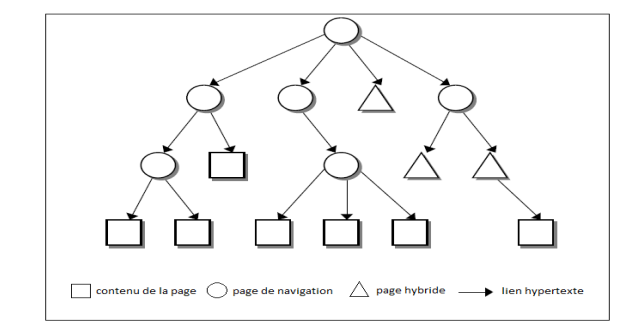
\includegraphics[width=0.7\textwidth]{images/filtrage base sur contenu.PNG}
    \caption{Structure en arbre d’un simple site web.PRES [Maarten et Someren, 2000]}
    \label{fig:structure_site}
\end{figure}
\paragraph{}
Un site Web peut être structuré en divisant ses pages web en des pages de contenu et des
pages de navigation (voir figure 2.2). Une page de contenu fournit à l'utilisateur les items
pertinents tandis qu’une page de navigation aide l’utilisateur à les rechercher. Les pages peuvent
également être hybrides, elles fournissent à la fois le contenu ainsi que des fonctionnalités de
navigation. Une page de navigation pour un utilisateur peut être une page de contenu pour un
autre et vice versa.
\paragraph{}
PRES traite les données et classifie les items dans une classe positive nommée C (items
pertinents). Par la suite il utilise les corrélations entre les contenus des items et les préférences
des utilisateurs pour déterminer le degré de similarité.
\paragraph{}
PRES affiche ses recommandations dynamiquement par la création des liens hypertextes
vers des pages de contenu qui contiennent les items pertinents. Il fait des recommandations en
comparant chaque profil d'utilisateur avec le contenu de chaque document de la collection. La
similarité entre le vecteur de profil et un document est déterminée par l’utilisation de la mesure
du cosinus dans un espace vectoriel <terme, contenu du site web>.
\paragraph{}
Quelques limites des systèmes de filtrage basé contenu sont présentées par Berrut et
Denos dans [Berrut et Denos, 2003]. La première difficulté pour ce type des systèmes c’est
qu’il ne traite que des documents textes, nous ne pouvons pas indexer des documents multimédia. De plus les systèmes basés contenu ne considèrent que le facteur thématique comme
critère de pertinence malgré qu’il existe d’autres facteurs tels que : la fiabilité de la source
d’information, la qualité scientifique et le degré de précision des faits présentés. Les auteurs
évoquent aussi l’effet « entonnoir » qui restreint le champ de vision de l’utilisateur: à force de ne
recommander que des items reliés à une seule et même thématique, et du fait que l’intérêt de
l’utilisateur est déterminé à partir des items choisis, on crée un effet d’auto-entraînement qui
restreint toujours plus la définition des intérêts de l’utilisateur et empêche l’exploration de
thématiques différentes.

\subsection{Le filtrage collaboratif}
Le filtrage collaboratif est un parmi les technologies les plus populaires dans le domaine des systèmes de recommandation \cite{Herlocker2000}. Le filtrage collaboratif se base sur l’idée que les personnes à la recherche d’information devraient se servir de ce que d’autres ont déjà trouvé et évalué. Dans la vie quotidienne, si quelqu’un a besoin d’une information, il essaye de s’informer généralement auprès de ses amis, ses collègues, qui vont à leurs tours lui recommander des articles, des films, des livres, etc. Cette collaboration entre les gens permet d’améliorer l’échange de connaissances, mais cela prend beaucoup de temps vu que cette ressource d’information ne peut pas toujours être à notre disposition. C’est à partir d’ici que l’idée de filtrage collaboratif est née, le besoin étant d’automatiser et de rendre l’échange des expériences et des avis personnels de certaines personnes utilisables par d’autres. Selon Golberg \cite{Golberg2001}, le filtrage collaboratif est l’automatisation des processus sociaux.

À la base du filtrage collaboratif, on utilise les choix explicites ou implicites des utilisateurs pour des items. Donc plutôt que d’utiliser une matrice termes-documents comme la recherche d’information le fait et comme l’approche basée sur le contenu, le filtrage collaboratif utilise la matrice des votes utilisateurs-items, où un vote peut être soit explicite (ex. fournir une cote à un film), soit implicite (ex. acheter un DVD du film).

Le tableau \ref{tab:matrice} illustre un exemple de matrice utilisateurs-items. Les valeurs peuvent représenter des votes ou des comportements. Dans cet exemple, l’item I3 n’a pas de vote pour l’utilisateur U1. On peut tenter de l’estimer soit avec une approche item-item ou une approche utilisateur-utilisateur comme expliqué dans les sections qui suivent.

\begin{table}[h!]
\centering
\caption{Matrice Items-utilisateurs}
\label{tab:matrice}
\begin{tabular}{|c|c|c|c|c|}
\hline
Utilisateur & Item I1 & Item I2 & Item I3 & Item I4 \\ \hline
U1         & 5       & 1       & ?       & 2       \\ \hline
U2         & 4       & 1       & 0       & 3       \\ \hline
U3         & 4       & 2       & 1       & 2       \\ \hline
U4         & 1       & 4       & 3       & 2       \\ \hline
\end{tabular}
\end{table}

Pour mieux définir ce type de filtrage, on se réfère aux travaux de Breese, Heckerman et Kadie dans [Breese, Heckerman et Kadie, 1998].. Ils décrivent plusieurs algorithmes conçus pour cette tâche, comprenant des techniques basées sur les coefficients de corrélation, le calcul de similarité basé sur les vecteurs et des méthodes bayésiennes statistiques. Le filtrage collaboratif peut prendre plusieurs formes : Item-Item et Utilisateur-Utilisateur.


\subsection{Filtrage item-item (Linden et al., 2003)}

Le filtrage item-item calcule la similarité des items dans la matrice utilisateur-items. Afin de déterminer les items les plus similaires à un item donné, cet algorithme construit un tableau des items similaires en cherchant les items populaires (que les clients ont tendance à acheter). Une matrice des produits entre les items est construite, ces produits représentant le degré de similarité entre les items (paire par paire). On peut trouver des paires qui n'ont aucun client en commun.

Dans le but de conserver le temps d'exécution et l'utilisation de la mémoire, il sera beaucoup mieux de calculer le produit d'un item par rapport aux autres items, au lieu de calculer les produits de tous les items à la fois.

La similarité entre les items peut être calculée de différentes méthodes, mais la méthode la plus commune est la mesure de cosinus des items.
\begin{figure}[h]
        \centering
        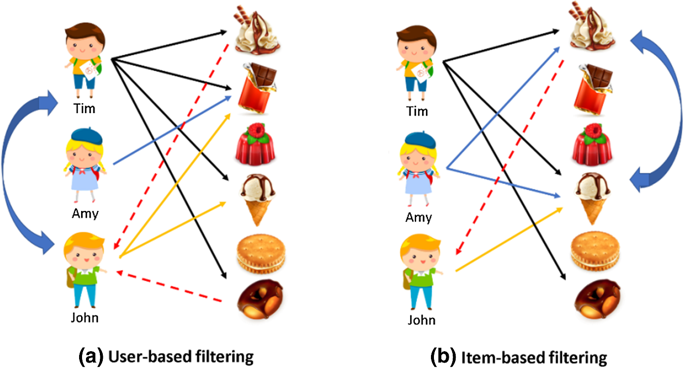
\includegraphics[width=0.8\textwidth]{images/item tem filtrage.png}
        \caption{Filtrage collaboratif basé sur les éléments.}
        \label{fig:classification}
\end{figure}

\subsection{Filtrage utilisateur-utilisateur}

Les filtres collaboratifs utilisent des bases de données sur les préférences des utilisateurs. Généralement, un utilisateur est caractérisé par ses goûts, ses préférences et ses choix, à travers ses traces (des achats, des consultations de pages, des votes, etc.). 

L'algorithme utilisateur-utilisateur cherche la similarité entre les profils des utilisateurs et recommande des items à un nouvel utilisateur. Ces recommandations sont basées sur le groupe le plus proche et le plus représentatif d’un individu. 

Le principe de cette approche est de chercher la similarité entre les profils utilisateurs en se basant sur leurs préférences et leurs appréciations.

Le tableau 1.2 représente les valeurs des votes donnés par quatre utilisateurs : U1, U2, U3 et U4, pour quatre items. L’utilisateur U1 n’a pas encore voté pour l’item I3. L’algorithme utilisateur-utilisateur permet d’estimer le vote de cet utilisateur U1 pour l’item I3 en fonction des votes des autres utilisateurs.

La valeur estimée $E$ de l'utilisateur U1 pour un item I3 est la somme pondérée des votes des autres utilisateurs $V_i$, qui ont des votes communs, où $i$ est l’index de chaque vote.

Ainsi, pour estimer le vote pour l’item I3, on utilise la formule suivante :

\[
v_{ij} = \text{moy}(v_i) + k \sum w_i v_i
\]

où :

\begin{itemize}
    \item $v_{ij}$ : vote de l’utilisateur $i$ pour l’item $j$,
    \item $\text{moy}(v_i)$ : vote moyen de l’utilisateur $i$,
    \item $k$ : constante pour normaliser la somme des $w_i$ à 1 (par exemple, si le poids est un cosinus, ce sera la somme des cosinus),
    \item $w_i$ : poids de l’utilisateur $i$ (ce poids peut être le cosinus entre le vecteur ligne de l’utilisateur pour lequel on désire estimer le vote et l’utilisateur $i$ ; cela peut aussi être la corrélation ou une autre mesure),
    \item $m$ : nombre de votes.
\end{itemize}
\subsection{Le filtrage hybride}

Le filtrage hybride combine les deux types de filtrage : basé sur le contenu et le filtrage collaboratif.
 
\section{Évaluation des systèmes de recommandation}

L’évaluation des systèmes de recommandation est cruciale pour mesurer leur efficacité et leur pertinence. Plusieurs méthodes existent pour évaluer les performances des algorithmes de recommandation. Ces méthodes peuvent être classées en différentes catégories selon le type de données, les objectifs de la recommandation, et la manière dont on mesure la qualité des recommandations. Nous détaillerons les principales méthodes utilisées pour évaluer ces systèmes.

\subsection{Mesures de précision des recommandations}

Les \textbf{mesures de précision} sont souvent utilisées pour évaluer la qualité des prédictions de score ou de note (rating) dans un système de recommandation.

\subsubsection{RMSE (Root Mean Squared Error)}
Le RMSE mesure l’erreur quadratique moyenne entre les valeurs prédites par le système et les valeurs réelles. La formule du RMSE est la suivante :
\[
RMSE = \sqrt{\frac{1}{N} \sum_{i=1}^{N} (y_i - \hat{y}_i)^2}
\]
où \(y_i\) représente la valeur réelle et \(\hat{y}_i\) la valeur prédite pour l’élément \(i\).

\textbf{Avantages :} Le RMSE pénalise fortement les grandes erreurs, ce qui est utile pour les systèmes où la précision des prédictions est essentielle.

\subsubsection{MAE (Mean Absolute Error)}
Le MAE est une autre mesure d'erreur, mais qui prend la moyenne des écarts absolus. Cette métrique est plus robuste que le RMSE lorsqu'il y a des erreurs très grandes.
\[
MAE = \frac{1}{N} \sum_{i=1}^{N} |y_i - \hat{y}_i|
\]
\textbf{Avantages :} MAE donne une idée générale de la moyenne des erreurs de prédiction.

\subsection{Mesures de classification des recommandations}

Les \textbf{mesures de classification} sont utilisées pour évaluer dans quelle mesure le système recommande des éléments pertinents.

\subsubsection{Précision (Precision)}
La précision mesure la proportion d'éléments correctement recommandés parmi tous ceux qui ont été recommandés par le système.
\[
Précision = \frac{\text{Nombre de recommandations correctes}}{\text{Nombre total de recommandations}}
\]
\textbf{Avantages :} La précision est utile pour les systèmes où il est important de recommander uniquement des éléments pertinents.

\subsubsection{Rappel (Recall)}
Le rappel mesure la proportion des éléments pertinents qui ont été recommandés parmi tous les éléments pertinents disponibles.
\[
Rappel = \frac{\text{Nombre de recommandations correctes}}{\text{Nombre total d'éléments pertinents}}
\]
\textbf{Avantages :} Le rappel est essentiel lorsque l’on veut minimiser les risques de ne pas recommander des éléments pertinents.

\subsubsection{F1-Score}
Le F1-score est la moyenne harmonique entre la précision et le rappel.
\[
F1 = 2 \times \frac{\text{Précision} \times \text{Rappel}}{\text{Précision} + \text{Rappel}}
\]
\textbf{Avantages :} Cette mesure combine à la fois la précision et le rappel, et est utilisée lorsqu’on veut un compromis entre les deux.

\subsection{Mesures de classement des recommandations}

Les \textbf{mesures de classement} évaluent la position des éléments pertinents dans la liste de recommandations.

\subsubsection{NDCG (Normalized Discounted Cumulative Gain)}
L’NDCG mesure l’efficacité d'un système en tenant compte de la position dans laquelle les éléments pertinents apparaissent. Un élément pertinent placé plus haut dans la liste est considéré comme plus utile.

\textbf{Avantages :} Permet d’évaluer les systèmes de recommandation en prenant en compte l’ordre des résultats.

\subsubsection{MRR (Mean Reciprocal Rank)}
Le MRR est une autre mesure de classement, qui se concentre sur la position du premier élément pertinent dans la liste. La formule est :
\[
MRR = \frac{1}{N} \sum_{i=1}^{N} \frac{1}{r_i}
\]
où \(r_i\) est la position du premier élément pertinent pour l’élément \(i\).

\textbf{Avantages :} Utilisé lorsque la priorité est donnée aux premiers éléments pertinents dans les recommandations.

\subsection{Autres critères d’évaluation}

Outre les métriques de précision et de classement, d’autres critères peuvent être pris en compte pour évaluer un système de recommandation.

\subsubsection{Couverture}
La couverture mesure la proportion d’éléments dans l'ensemble total qui peuvent être recommandés par le système.

\textbf{Avantages :} Permet de voir si le système couvre bien une large gamme de produits ou services.

\subsubsection{Diversité}
La diversité évalue si le système recommande des éléments variés ou s’il se limite à recommander des éléments similaires.

\textbf{Avantages :} Une bonne diversité évite la monotonie et augmente l’expérience utilisateur.

\subsubsection{Nouveauté}
La nouveauté mesure dans quelle mesure les éléments recommandés sont nouveaux pour l'utilisateur, c'est-à-dire qu’ils ne sont pas encore connus.

\textbf{Avantages :} Permet d’éviter de simplement recommander les éléments populaires, mais plutôt de surprendre l'utilisateur avec des nouveautés.

\section{Limites des systèmes de recommandation}

Malgré les progrès réalisés dans le domaine des systèmes de recommandation, plusieurs défis et limitations subsistent. Ces limitations peuvent affecter la performance des systèmes, leur capacité à personnaliser les recommandations et l’expérience utilisateur. Parmi les principales limites, on trouve les problèmes du \textit{cold start}, de la \textit{sparsité}, et du \textit{sur-apprentissage}. Nous détaillons ces limitations ci-dessous.

\subsection{Problème du Cold Start}

Le \textit{cold start} est un problème majeur qui survient lorsque le système de recommandation doit générer des recommandations pour un utilisateur ou un produit nouvellement ajouté au système, pour lesquels il n'existe pas encore suffisamment de données historiques. Ce problème peut être divisé en trois catégories principales :

\begin{itemize}
    \item \textbf{Cold start utilisateur :} Lorsque de nouveaux utilisateurs s'inscrivent dans le système, il n'y a pas de données sur leurs préférences ou comportements passés, ce qui rend difficile la génération de recommandations pertinentes. Cela peut entraîner une expérience utilisateur moins satisfaisante.
    \item \textbf{Cold start produit :} De nouveaux produits ou articles ajoutés au catalogue du système ne bénéficient pas encore d'évaluations ou de comportements d'utilisateur, ce qui les rend difficiles à recommander.
    \item \textbf{Cold start général :} Lorsque les deux (utilisateur et produit) sont nouveaux, le système fait face à un problème de manque de données pour établir des liens ou des similarités entre utilisateurs et produits.
\end{itemize}

\textbf{Solutions possibles :} Certaines approches pour atténuer le problème du cold start incluent l’utilisation de techniques de recommandation hybride, où les données externes (comme les informations démographiques des utilisateurs ou les caractéristiques des produits) sont utilisées pour combler le manque d'information.

\subsection{Problème de Sparsité}

La \textit{sparsité} fait référence à la situation dans laquelle la matrice de notation utilisateur-produit contient un grand nombre de valeurs manquantes. Autrement dit, la majorité des utilisateurs n'ont pas évalué tous les produits disponibles. Cela rend difficile l’identification de similarités fiables entre utilisateurs ou produits, ce qui affecte la qualité des recommandations.

\begin{itemize}
    \item \textbf{Exemple de sparsité :} Dans un grand catalogue de films, un utilisateur peut ne noter que quelques films, tandis qu'il y en a des milliers disponibles. Si la majorité des utilisateurs évaluent seulement une petite fraction des films, la matrice de notation devient extrêmement clairsemée, rendant les algorithmes de recommandation traditionnels moins efficaces.
\end{itemize}

\textbf{Solutions possibles :} Pour résoudre ce problème, certaines techniques comme la \textit{factorisation matricielle} ou l’utilisation d'approches basées sur \textit{les voisins les plus proches} peuvent être employées pour estimer les évaluations manquantes et rendre les systèmes plus efficaces.

\subsection{Problème de Sur-apprentissage (Overfitting)}

Le \textit{sur-apprentissage} survient lorsqu’un modèle de recommandation apprend trop bien les spécificités des données d’entraînement, au point qu'il ne généralise pas bien aux nouvelles données. Cela peut entraîner une sur-optimisation des recommandations pour les utilisateurs ou les produits déjà présents dans le jeu de données, mais une mauvaise performance sur les nouveaux utilisateurs ou produits.

\begin{itemize}
    \item \textbf{Exemple de sur-apprentissage :} Si un système de recommandation devient trop spécifique en se basant sur des préférences utilisateurs très précises, il risque de ne pas être capable de recommander des éléments pour des utilisateurs avec des comportements différents.
\end{itemize}

\textbf{Solutions possibles :} Pour éviter le sur-apprentissage, il est essentiel d’utiliser des techniques de régularisation, de validation croisée, et de prendre en compte la diversité des recommandations. L’utilisation de modèles plus simples ou de méthodes hybrides peut également aider à limiter ce problème.

\subsection{Problème du Biais et de la Diversité}

Le biais dans les systèmes de recommandation survient lorsque le modèle favorise certaines préférences ou types de produits au détriment d'autres, souvent en raison d'un manque de diversité dans les données d'entraînement ou des algorithmes de recommandation. Cela peut conduire à des recommandations trop homogènes ou centrées sur des articles populaires.

\begin{itemize}
    \item \textbf{Exemple de biais :} Si un système de recommandation se concentre uniquement sur les produits populaires ou les articles déjà évalués, il pourrait ne pas offrir des recommandations suffisamment variées, limitant ainsi l’expérience de l’utilisateur.
\end{itemize}

\textbf{Solutions possibles :} Pour surmonter ce problème, des techniques comme l’introduction de \textit{diversité} dans les algorithmes ou l’utilisation de modèles de recommandation qui intègrent des critères de nouveauté peuvent être appliquées. L'injection de la diversité dans les résultats peut ainsi améliorer l’expérience utilisateur et éviter les biais.

\subsection{Problème de Scalabilité}

Les systèmes de recommandation doivent traiter de grandes quantités de données, en particulier dans des environnements de grande échelle tels que les plateformes de commerce en ligne. Le problème de scalabilité se pose lorsque le système de recommandation peine à maintenir sa performance à mesure que la taille de l’ensemble des utilisateurs et des produits augmente.

\begin{itemize}
    \item \textbf{Exemple de scalabilité :} Un système de recommandation peut devenir lent ou inefficace à mesure que le nombre d’utilisateurs ou de produits augmente. Le temps de calcul des recommandations peut devenir prohibitif.
\end{itemize}

\textbf{Solutions possibles :} Les solutions à ce problème incluent l’utilisation de techniques d'optimisation, telles que la \textit{parallélisation} des calculs ou l'utilisation de \textit{l'informatique distribuée}, ainsi que des modèles approximatifs qui permettent de réduire la charge computationnelle.

\subsection{Problème d'Évaluation et de Mesure}

L’évaluation des systèmes de recommandation est également un défi. Les mesures traditionnelles, telles que la précision ou le rappel, ne tiennent pas toujours compte des nuances des préférences des utilisateurs, comme la diversité ou la nouveauté. De plus, la mesure de la satisfaction de l’utilisateur peut être subjective et difficile à quantifier de manière objective.

\textbf{Solutions possibles :} L’utilisation de métriques combinées telles que le F1-score ou de mesures spécifiques aux applications, comme le NDCG (Discounted Cumulative Gain), permet d’évaluer plus précisément la pertinence des recommandations.
